\documentclass[letterpaper]{article}

\usepackage[english]{babel}
\usepackage[utf8]{inputenc}
\usepackage{amsmath}
\usepackage{graphicx}
\usepackage[colorinlistoftodos]{todonotes}
\usepackage[]{algorithm2e}
\usepackage{listings}
\usepackage{hyperref}
\usepackage{float}
\usepackage{afterpage}

\title{CSCE 636: Homework 1}

\author{Aryan Sharma\\UIN: 326006767} % The article author(s) - author affiliations need to be specified in the AUTHOR AFFILIATIONS block

\date{} % An optional date to appear under the author(s)

\begin{document}
	
\maketitle

\noindent {\Large Question 1}\\

\noindent \textbf{1a.} The function train\_valid\_split, splits the dataset into training and validation sets. The training dataset is the actual dataset that we use to train the model. However, if we use the entire training dataset, we can overfit and may not generalize well to the test data. The validation dataset is thus used to tune the hyperparameters. By testing on a set of validation examples that the models were not trained on, we obtain a better estimate of each hypothesis hi’s true gene\\

\noindent \textbf{1b.} We can use the full dataset to produce our final model as the more data we use the more likely it is to generalise well but we should also make sure that we obtain an unbiased performance estimate via nested cross-validation and potentially consider penalising the cross-validation statistic to further avoid over-fitting in model selection.\\

\noindent \textbf{1c.} Implemented in code\\

\noindent \textbf{1d.} This is to take into account the bias while taking the product so that we can do vectorized operations.\\

\noindent \textbf{1e.} Implemented in code\\

\noindent \textbf{1f.} Shown in Fig. 1\\\\

 \begin{figure}
 	\centering
	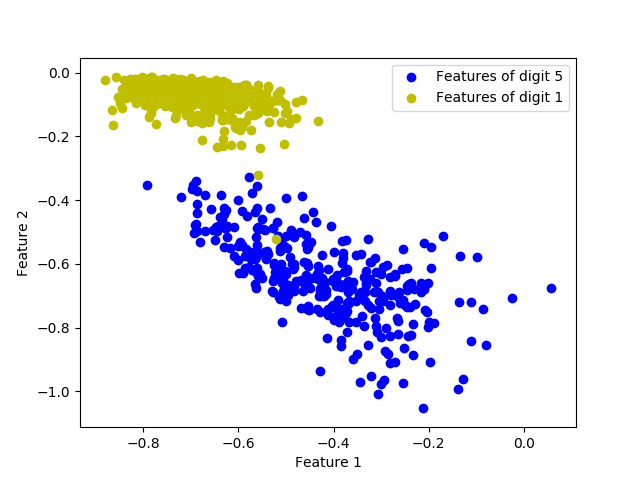
\includegraphics[width=0.8\textwidth]{train_features_img0.png}
	\caption{\label{fig:data}Training Data Features}
\end{figure}

\noindent {\Large Question 2}\\

\noindent \textbf{2a.} Implemented in code\\

\noindent \textbf{2b.} Implemented in code\\

\noindent \textbf{2c.} Shown in Fig. 2\\

 \begin{figure}
	\centering
	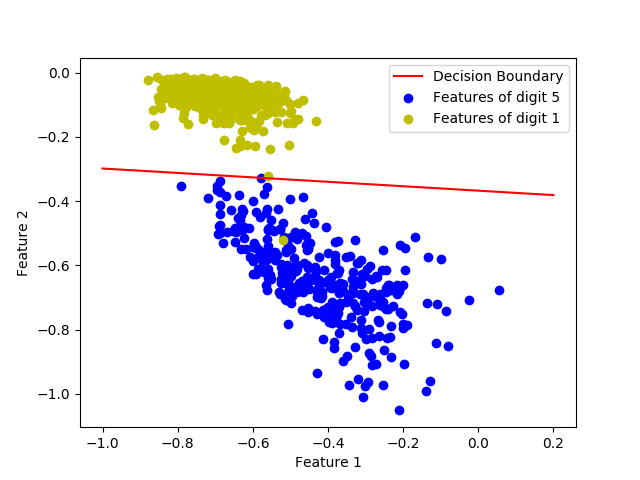
\includegraphics[width=0.8\textwidth]{test_features_img1.png}
	\caption{\label{fig:data}Test Data Features and Decision Line for Perceptron Learning}
\end{figure}

\noindent \textbf{2d.} Implemented in code. The test accuracy is 98.35\%.

\noindent {\Large Question 3}\\

\noindent \textbf{3a.} The loss function for Logistic Regression is generated by maximizing the log likelihood of the probability of getting they \(1,...,y_N\) in \(D\) from the corresponding \(x_1,...,x_N\): 
\[\max P(y_1,....y_N | x_1,...,x_N)\]
\[= \max \prod_{n=1}^{N} P(y_n|x_n)\]
\[\rightleftharpoons\max log(\prod_{n=1}^{N} P(y_n|x_n))\]
\[= \max \sum_{n=1}^{N} log(P(y_n|x_n)\]
\[\rightleftharpoons\min -\frac{1}{N} \sum_{n=1}^{N} log(P(y_n|x_n)\]
\[= \min \frac{1}{N} \sum_{n=1}^{N} log(\frac{1}{P(y_n|x_n})\]
\[= \min \frac{1}{N} \sum_{n=1}^{N} log(\frac{1}{\sigma(y_n.W^Tx_n)})\]
\[= \min \frac{1}{N} \sum_{n=1}^{N} log(1+e^{-y_n.W^Tx_n})\]

Hence the loss function for one training example is \[E(W) = \sum_{n=1}^{N} log(1+e^{-y_n.W^Tx_n})\]\\

\noindent \textbf{3b.} Gradient of \(E(w) = -y_ix_i/(1+e^{-y_i.W^Tx_i})\)\\

\[\nabla E(w) = \frac{\partial }{\partial W} log(1+e^{-y_i.W^Tx_i})\]
\[= \frac{1}{1+e^{-y_i.W^Tx_i}} \frac{\partial }{\partial W} (1+e^{-y_i.W^Tx_i})\]
\[= \frac{ -y_ix_i}{1+e^{-y_i.W^Tx_i}}\]\\

\noindent \textbf{3c.} The linear line of seperation fails to capture the complex non-linear variations in real life data and misclassifies more data points than a non-linear surface of separation. Hence it is inefficient. The sigmoid layer is used when we want to convert our prediction into probabilities ie. between 0 and 1.\\

\noindent \textbf{3d.} Yes, the decision boundary is still linear. This is because the boundary is still a linear function separating data points where \(\theta (w^Tx)\) is \(0.9\). \\

\noindent \textbf{3e.} Logistic regression is considered a generalized linear model. This is because the outcome always depends on the additivity of the inputs and parameters and not on the product (or quotient, etc.) of its parameters. \\\\

\noindent {\Large Question 4}\\

\noindent \textbf{4a.} Implemented in code.\\

\noindent \textbf{4b.} Implemented in code.\\

\noindent \textbf{4c.} Implemented in code.\\

\noindent \textbf{4d.} Implemented in code. The visualization of features is shown in Fig 3.\\

 \begin{figure}
	\centering
	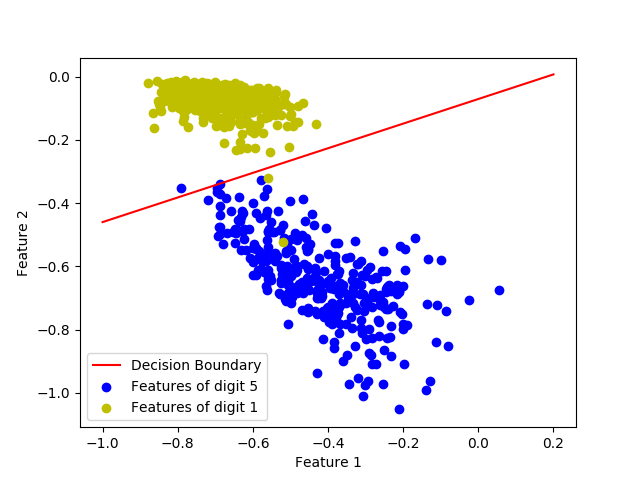
\includegraphics[width=0.8\textwidth]{test_features_img4.png}
	\caption{\label{fig:data}Test Data Features and Decision Line for Losgistic Regression Model}
\end{figure}

\noindent \textbf{4e.} The hyperparameters earning rate and maximum iterations were tuned. The analysis is shown in Fig 4. and Fig 5. The test accuracy is 98.95\%

 \begin{figure}
	\centering
	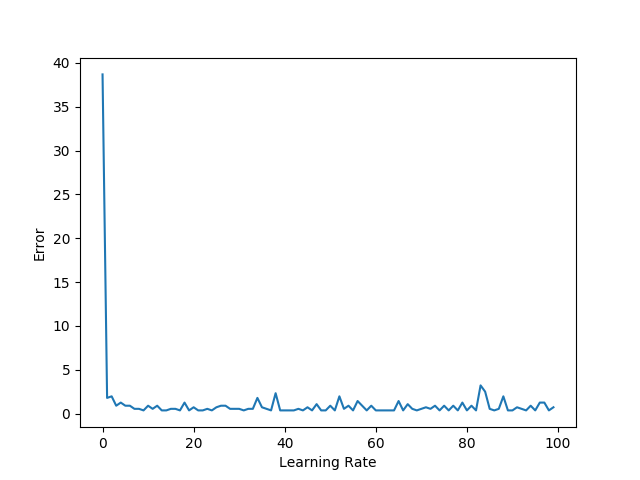
\includegraphics[width=0.8\textwidth]{variation_learning_rate_img2.png}
	\caption{\label{fig:data} Tuning the learning rate}
\end{figure}

 \begin{figure}
	\centering
	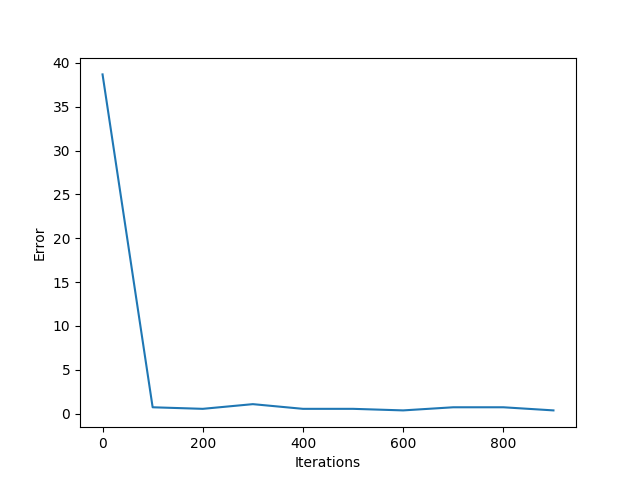
\includegraphics[width=0.8\textwidth]{variation_max_iters_img3.png}
	\caption{\label{fig:data} Tuning the maximum iterations}
\end{figure}

\end{document}